\section{Comportement}
\label{sec:Comportement}
Concernant les blessures préalablement observées lors du stage de B. SOMON, aucune n'a pu être reproduite durant mon stage. Les animaux ont cependant été qualifiés de "bien plus sensible à leurs environnement que la normale" par les animaliers en charges de ceux-ci. On peut alors penser que durant le stage précédent, comme l'animalerie n'était pas la même, les animaux étaient soumis à un stress plus importants, et adoptaient comme réponse à ce stress un comportement d'automutilation. \todo{Bof. A remanier}

\section{Structure du cerveau}
\label{sec:NisslResultat}
La coloration de Nissl à base de Crésyl violet est une marquage classique du tissu nerveux, qui marque l'acide nucléique des cellules car chargé négativement. Ce marquage cible particulièrement les neurones, riches en réticulum endoplasmique rugueux, résultant en la présence d'une grande quantité d'\acrshort{arn}. Cette coloration permet de mettre en évidence les motifs des structures cellulaires.

Afin de visualiser si la mutation \mcrd altérait l'organisation structurale du cerveau, une coloration de Nissl a été réalisée (\cref{fig:NisslResultat}). Cette coloration a permis de mettre en évidence que la mutation n'altérait pas de manière visible l'organisation du cerveau, à la fois chez les souris femelles (\cref{fig:FemWTNissl,fig:FemMutNissl}) et mâles(\cref{fig:MaleWTNissl,fig:MaleMutNissl}) .

\begin{figure}[h] %Figure Nissl Résultats
	\begin{center}
		\begin{subfigure}[h]{0.49\textwidth}%F437 WT Nissl 33 l2.tif
			\caption{}
			\label{fig:FemWTNissl}
			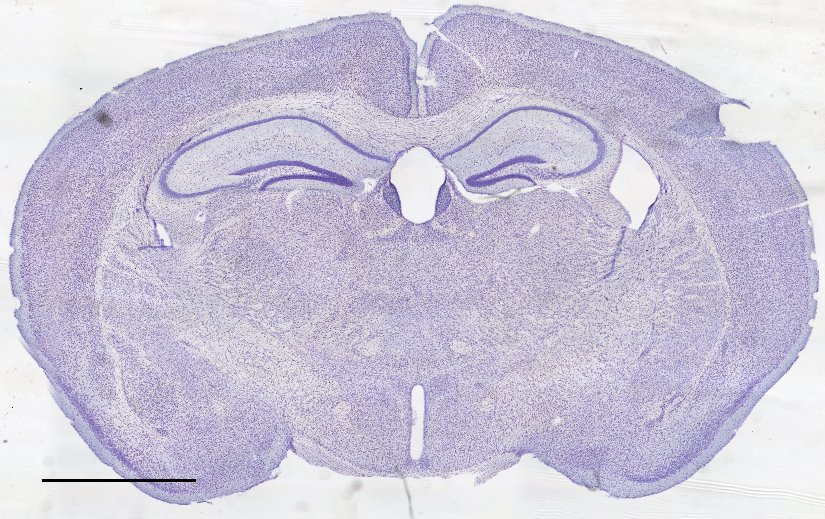
\includegraphics[width=\textwidth]{./Images/Nissl/FemWT.jpg}
		\end{subfigure}
		\begin{subfigure}[h]{0.49\textwidth}%F435 Mut Nissl 38.tif
			\caption{}
			\label{fig:FemMutNissl}
			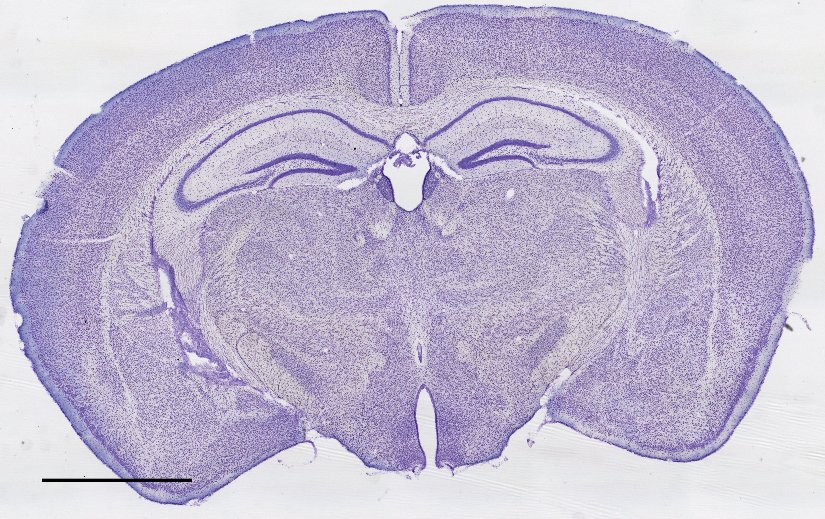
\includegraphics[width=\textwidth]{./Images/Nissl/FemMut.jpg}
		\end{subfigure}
		\begin{subfigure}[h]{0.49\textwidth}%M2 WT Nissl #031.tif
			\caption{}
			\label{fig:MaleWTNissl}
			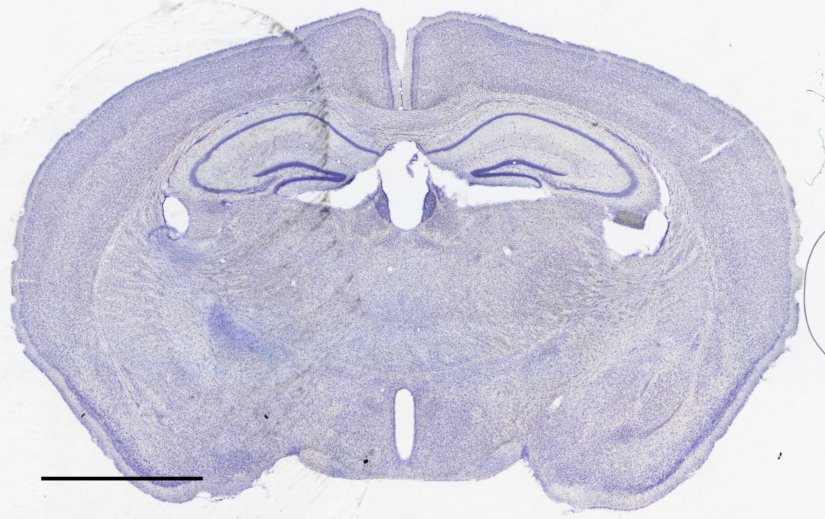
\includegraphics[width=\textwidth]{./Images/Nissl/MaleWT.jpg}
		\end{subfigure}
		\begin{subfigure}[h]{0.49\textwidth}%M442 Mut Nissl lame 3 36.tif
			\caption{}
			\label{fig:MaleMutNissl}
			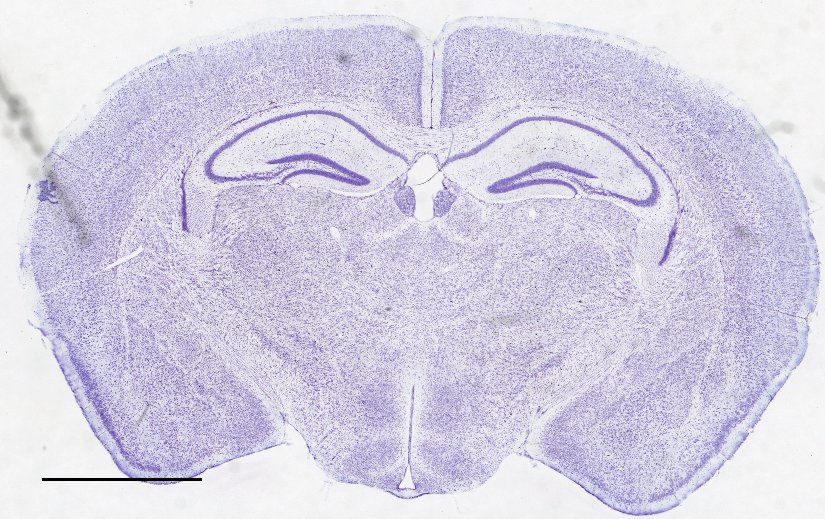
\includegraphics[width=\textwidth]{./Images/Nissl/MaleMut.jpg}
		\end{subfigure}
	\end{center}
	\caption{Coloration de Nissl}
	\descfig{\subref{fig:FemWTNissl} Femelle sauvage. \subref{fig:FemMutNissl} Femelle mutante. \subref{fig:MaleWTNissl} Mâle sauvage. \subref{fig:MaleMutNissl} Mâle mutant. Images représentatives centrées autour de la région autour de l'hippocampe. Âge moyen des souris : 30 jours. Barre d'échelle : 2 mm.}
	\label{fig:NisslResultat}
\end{figure}
%\FloatBarrier

\section{Immunomarquage}

\section{Immunoprécipitation}
\label{sec:IPresultat}
Afin de confirmer la détection de \gls{musk} dans diverse région du cerveau, une immunoprécipitation suivie d'un \gls{wb} a été réalisée sur l'hippocampe, le cervelet et le cortex de trois souris C57Bl/6 sauvage. Un \gls{wb} de \gls{musk} a déjà été décrit sur des diverses struFloatBarrier
ctures du cerveau \cite{Garcia-Osta2006}, mais à partir d'extrait totale. Durant son stage, B. SOMON a tentée de réaliser un \gls{ip} suivi d'un \gls{wb}, mais sans obtenir de résultats probant. Ici, la principale modification apportée au protocole est l'utilisation de tampon RIPA (adjonction de déoxycholate de sodium et de \acrshort{sds}) lors de l'extraction des protéines.

\begin{wrapfigure}{l}{0.45\textwidth}[h]
	\missingfigure{WB musk : c'est joli, hein ?}
	\caption{WB après IP}{On peut observer ici...rien du tout !}
	\label{fig:WBMuSK}
\end{wrapfigure}

%\section{Expression de \gls{musk}}